% Presentación de la defensa del TFM VeriVoto.
% Compilar desde esta carpeta: pdflatex presentacion.tex (dos veces). Las figuras se toman de la memoria
% (../Plantilla-TFM-Informatica-UAL/Figuras), así que un cambio en un diagrama de la memoria llega aquí solo.
% Guion de cada diapositiva: guion.md. Preguntas previsibles del tribunal: preguntas.md.
\documentclass[aspectratio=169,11pt]{beamer}
\usepackage[utf8]{inputenc}
\usepackage[T1]{fontenc}
\usepackage[spanish,es-noshorthands]{babel}
\usepackage{booktabs}
\usepackage{array}
\usepackage{appendixnumberbeamer} % la reserva no cuenta en el total de diapositivas
\usepackage{estilo-ual}

\graphicspath{{../Plantilla-TFM-Informatica-UAL/Figuras/}}
\newcommand{\diagrama}[1]{\input{../Plantilla-TFM-Informatica-UAL/Figuras/diagramas/#1.tex}}

\title[VeriVoto]{VeriVoto: diseño e implementación de una plataforma SaaS de votación digital segura y auditable para organizaciones}
\subtitle{Arquitectura cloud multi-tenant y API abierta}
\author[Saul David Ramos Pacheco]{Saul David Ramos Pacheco}
\institute{Máster Universitario en Ingeniería Informática\\Universidad de Almería\\[3pt]Director: Javier Criado Rodríguez}
\date{Defensa del Trabajo Fin de Máster · Curso 2026/2027}

\begin{document}

% ---------------------------------------------------------------- 1
{
\setbeamertemplate{footline}{}
\begin{frame}[plain]
  \begin{tikzpicture}[remember picture,overlay]
    \fill[ualturquesa] (current page.north west) rectangle ([yshift=-0.9cm]current page.north east);
    \node[anchor=north west,text=white,font=\bfseries\small,inner sep=8pt] at (current page.north west)
      {TRABAJO FIN DE MÁSTER};
    \node[anchor=south east,inner sep=10pt] at (current page.south east)
      {
\includegraphics[height=1.6cm]{logos/escudocolor.png}};
  \end{tikzpicture}
  \vspace{1.2cm}
  {\color{ualoscuro}\Large\bfseries VeriVoto\par}
  \vspace{4pt}
  {\large Diseño e implementación de una plataforma SaaS de votación digital segura y auditable para organizaciones, con arquitectura cloud multi-tenant y API abierta\par}
  \vspace{14pt}
  {\normalsize\bfseries Saul David Ramos Pacheco\par}
  {\small Director: Javier Criado Rodríguez\par}
  \vspace{8pt}
  {\footnotesize Máster Universitario en Ingeniería Informática · Universidad de Almería · Curso 2026/2027\par}
\end{frame}
}

% ---------------------------------------------------------------- 2
\section{Problema}
\begin{frame}{Problema y motivación}
  \begin{columns}[T]
    \column{0.55\textwidth}
    Universidades, asociaciones y organizaciones celebran \textbf{votaciones internas} frecuentes:
    representantes, juntas, consultas.
    \begin{itemize}
      \item Papel o formularios genéricos: sin secreto real ni control de duplicados.
      \item Plataformas comerciales: cerradas, de pago por elección y sin API.
      \item Soluciones académicas verificables: difíciles de entender para un votante no técnico.
    \end{itemize}
    \column{0.42\textwidth}
    \textbf{Lo que se necesita}
    \begin{itemize}
      \item Secreto y \textbf{un voto por persona}
      \item Evidencia que el votante entienda
      \item Auditoría del recuento
      \item Uso desde el móvil y accesible
      \item Varias organizaciones en una plataforma
    \end{itemize}
  \end{columns}
\end{frame}

% ---------------------------------------------------------------- 3
\begin{frame}{Estado del arte: huecos detectados}
  \footnotesize
  \begin{tabular}{@{}>{\raggedright\arraybackslash}p{0.27\textwidth}>{\raggedright\arraybackslash}p{0.30\textwidth}>{\raggedright\arraybackslash}p{0.35\textwidth}@{}}
    \toprule
    \textbf{Tipo} & \textbf{Ejemplos} & \textbf{Limitación para este caso}\\
    \midrule
    SaaS comerciales & ElectionBuddy, Simply Voting, OpaVote, POLYAS & Coste por elección, API limitada o de pago, verificación poco explicada \\
    Código abierto verificable & Helios, Belenios & Criptografía difícil de explicar; sin multi-organización ni SSO institucional \\
    Participación ciudadana & Decidim, Vocdoni & Orientadas a procesos públicos, no a la votación interna sencilla \\
    \bottomrule
  \end{tabular}
  \vspace{10pt}
  \ualbloque{\small \textbf{Hueco:} autenticación institucional, experiencia móvil accesible y una \textbf{verificación comprensible}, en un servicio multi-organización con API abierta.}
\end{frame}

% ---------------------------------------------------------------- 4
\section{Objetivos}
\begin{frame}{Objetivos y preguntas de investigación}
  \begin{columns}[T]
    \column{0.52\textwidth}
    \textbf{Objetivos}
    \begin{description}\footnotesize
      \item[OBJ-1] Arquitectura SaaS multi-tenant, identidad y roles
      \item[OBJ-2] Censo, ciclo de vida de votaciones y API documentada
      \item[OBJ-3] Participación accesible con secreto, unicidad y recibo comprensible
      \item[OBJ-4] Escrutinio, trazabilidad y actas; calidad según ISO/IEC 25010:2023
    \end{description}
    \column{0.45\textwidth}
    \textbf{Preguntas}
    \begin{description}\footnotesize
      \item[RQ1] ¿Cómo hacer la verificación comprensible para usuarios no técnicos?
      \item[RQ2] ¿Qué separación entre identidad y urna protege el secreto y la unicidad?
      \item[RQ3] ¿Cómo evaluar la calidad con ISO/IEC 25010:2023?
    \end{description}
  \end{columns}
\end{frame}

% ---------------------------------------------------------------- 5
\begin{frame}{Metodología y alcance}
  \begin{columns}[T]
    \column{0.5\textwidth}
    \textbf{Design Science Research}
    \begin{itemize}\small
      \item Problema \(\rightarrow\) artefacto \(\rightarrow\) evaluación
      \item Hitos P0--P9 con diagrama de Gantt
      \item Prioridades MoSCoW y decisiones registradas (D-xx)
      \item Hipótesis con criterio fijado \textbf{antes} de medir
    \end{itemize}
    \column{0.47\textwidth}
    \textbf{Alcance del MVP}
    \begin{itemize}\small
      \item RF-01 a RF-21 implementados
      \item Fuera: sustituir el voto (RF-11), métodos avanzados (RF-22), cifrado en cliente (RF-23)
      \item Actores: superadministrador, administración, gestión de censo, auditoría y votante
      \item Evaluado en local con datos sintéticos (no desplegado)
    \end{itemize}
  \end{columns}
\end{frame}

% ---------------------------------------------------------------- 6
\section{Arquitectura}
\begin{frame}{Arquitectura implementada}
  \centering
  \resizebox{!}{0.78\textheight}{\diagrama{arquitectura_implementada}}\\[2pt]
  \footnotesize Java 25 + Spring Boot (hexagonal) · Angular/Ionic (PWA) · Keycloak 26 · PostgreSQL 18 · REST + \emph{outbox}
\end{frame}

% ---------------------------------------------------------------- 7
\begin{frame}{Secreto del voto: separar identidad y urna}
  \begin{columns}[T]
    \column{0.36\textwidth}
    \footnotesize
    \begin{itemize}
      \item \textbf{voter-access} sabe \emph{quién} participa, solo con el día.
      \item \textbf{ballot-box} guarda \emph{qué} se vota, sin identidad ni hora.
      \item Un \textbf{token de un solo uso} une los dos pasos: 20 intentos simultáneos dan 1 voto.
      \item Bases de datos separadas (\texttt{pg-ballot}).
    \end{itemize}
    \ualbloque{\footnotesize Límite: no protege frente a quien controle a la vez las dos bases o el dispositivo.}
    \column{0.62\textwidth}
    \centering
    \resizebox{!}{0.80\textheight}{\diagrama{secuencia_emitir_voto_recibo}}
  \end{columns}
\end{frame}

% ---------------------------------------------------------------- 8
\begin{frame}{Recibo y auditoría}
  \begin{columns}[T]
    \column{0.5\textwidth}
    \textbf{Para el votante}
    \begin{itemize}\small
      \item Recibo de 64 caracteres tras votar
      \item Página pública: «tu voto consta en la urna»
      \item Nunca muestra la opción elegida
    \end{itemize}
    \column{0.47\textwidth}
    \textbf{Para la auditoría}
    \begin{itemize}\small
      \item Cada evento de la urna se encadena con una huella SHA-256
      \item Huella final pública; escrutinio bloqueado si la cadena se rompe
      \item El resultado se recalcula en el navegador
      \item Acta PDF con su huella
    \end{itemize}
  \end{columns}
  \vspace{8pt}
  \ualbloque{\small Acredita \textbf{presencia e integridad}; no es verificabilidad extremo a extremo (fuera de alcance, RF-23).}
\end{frame}

% ---------------------------------------------------------------- 9
\section{Prototipo}
\begin{frame}{El prototipo}
  \begin{columns}[T]
    \column{0.5\textwidth}\centering
    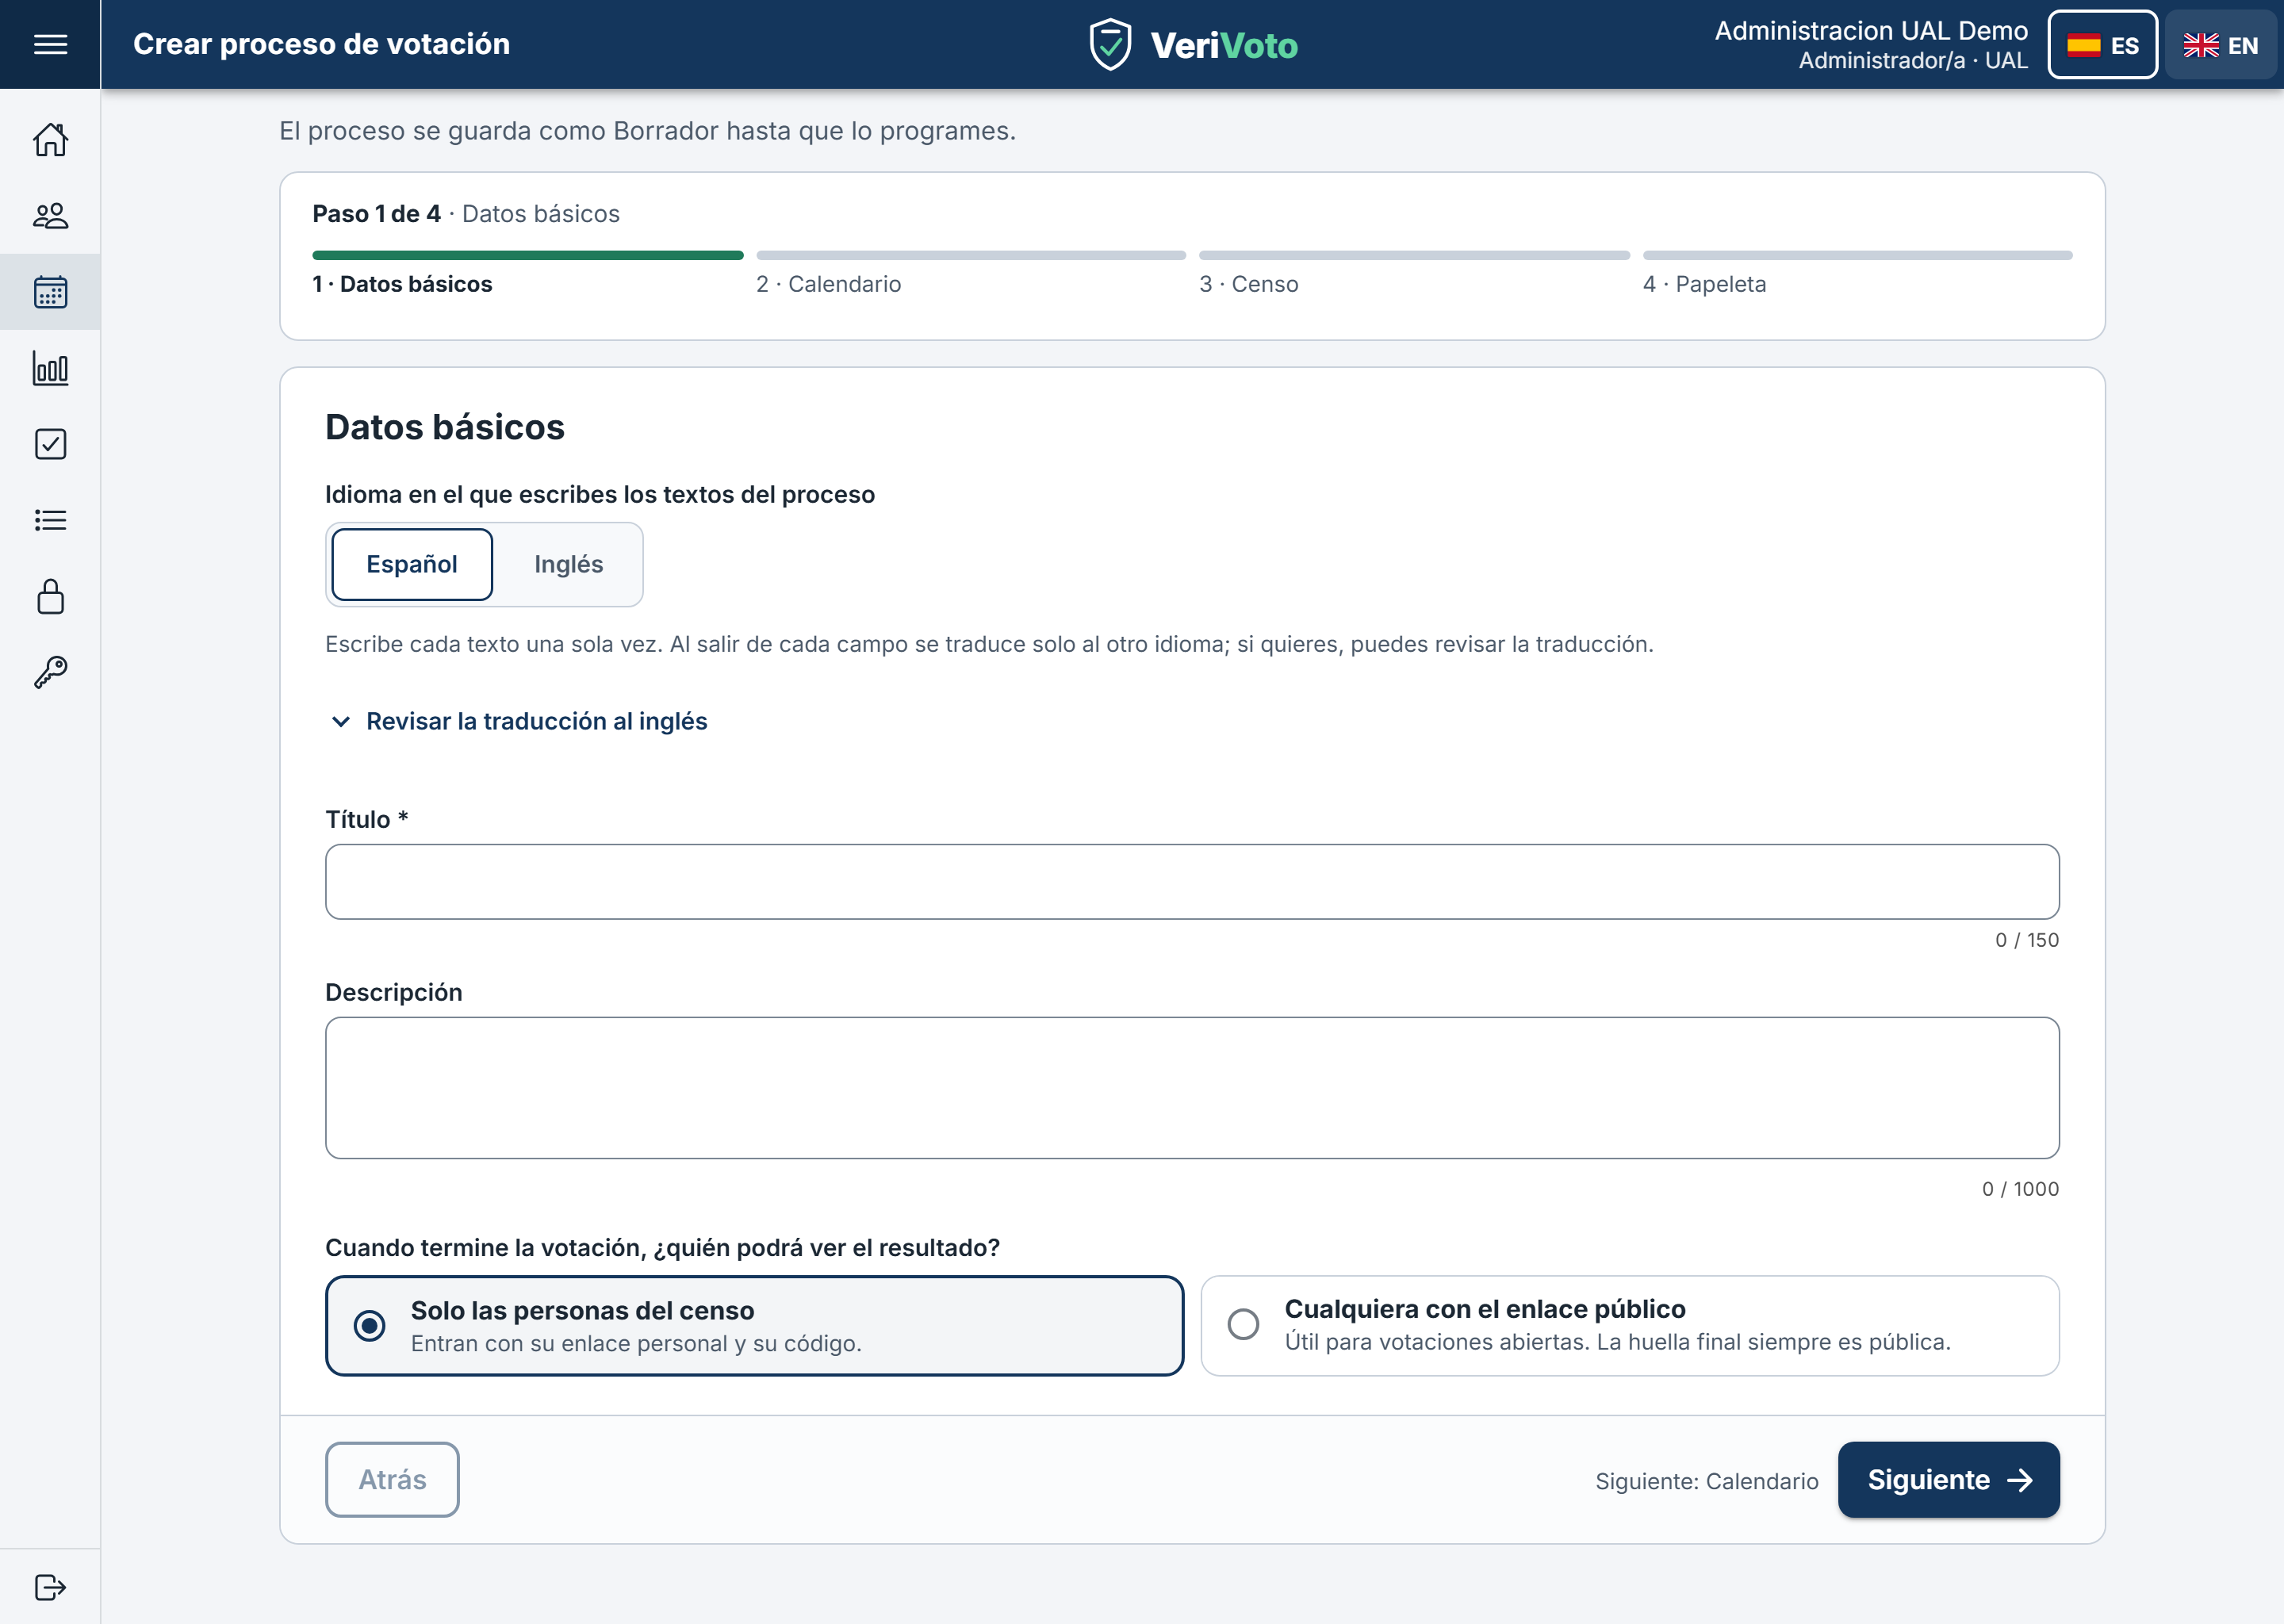
\includegraphics[width=\linewidth]{capturas/consola-proceso-nuevo-es}\\
    \footnotesize Asistente de creación (RF-06)
    \column{0.5\textwidth}\centering
    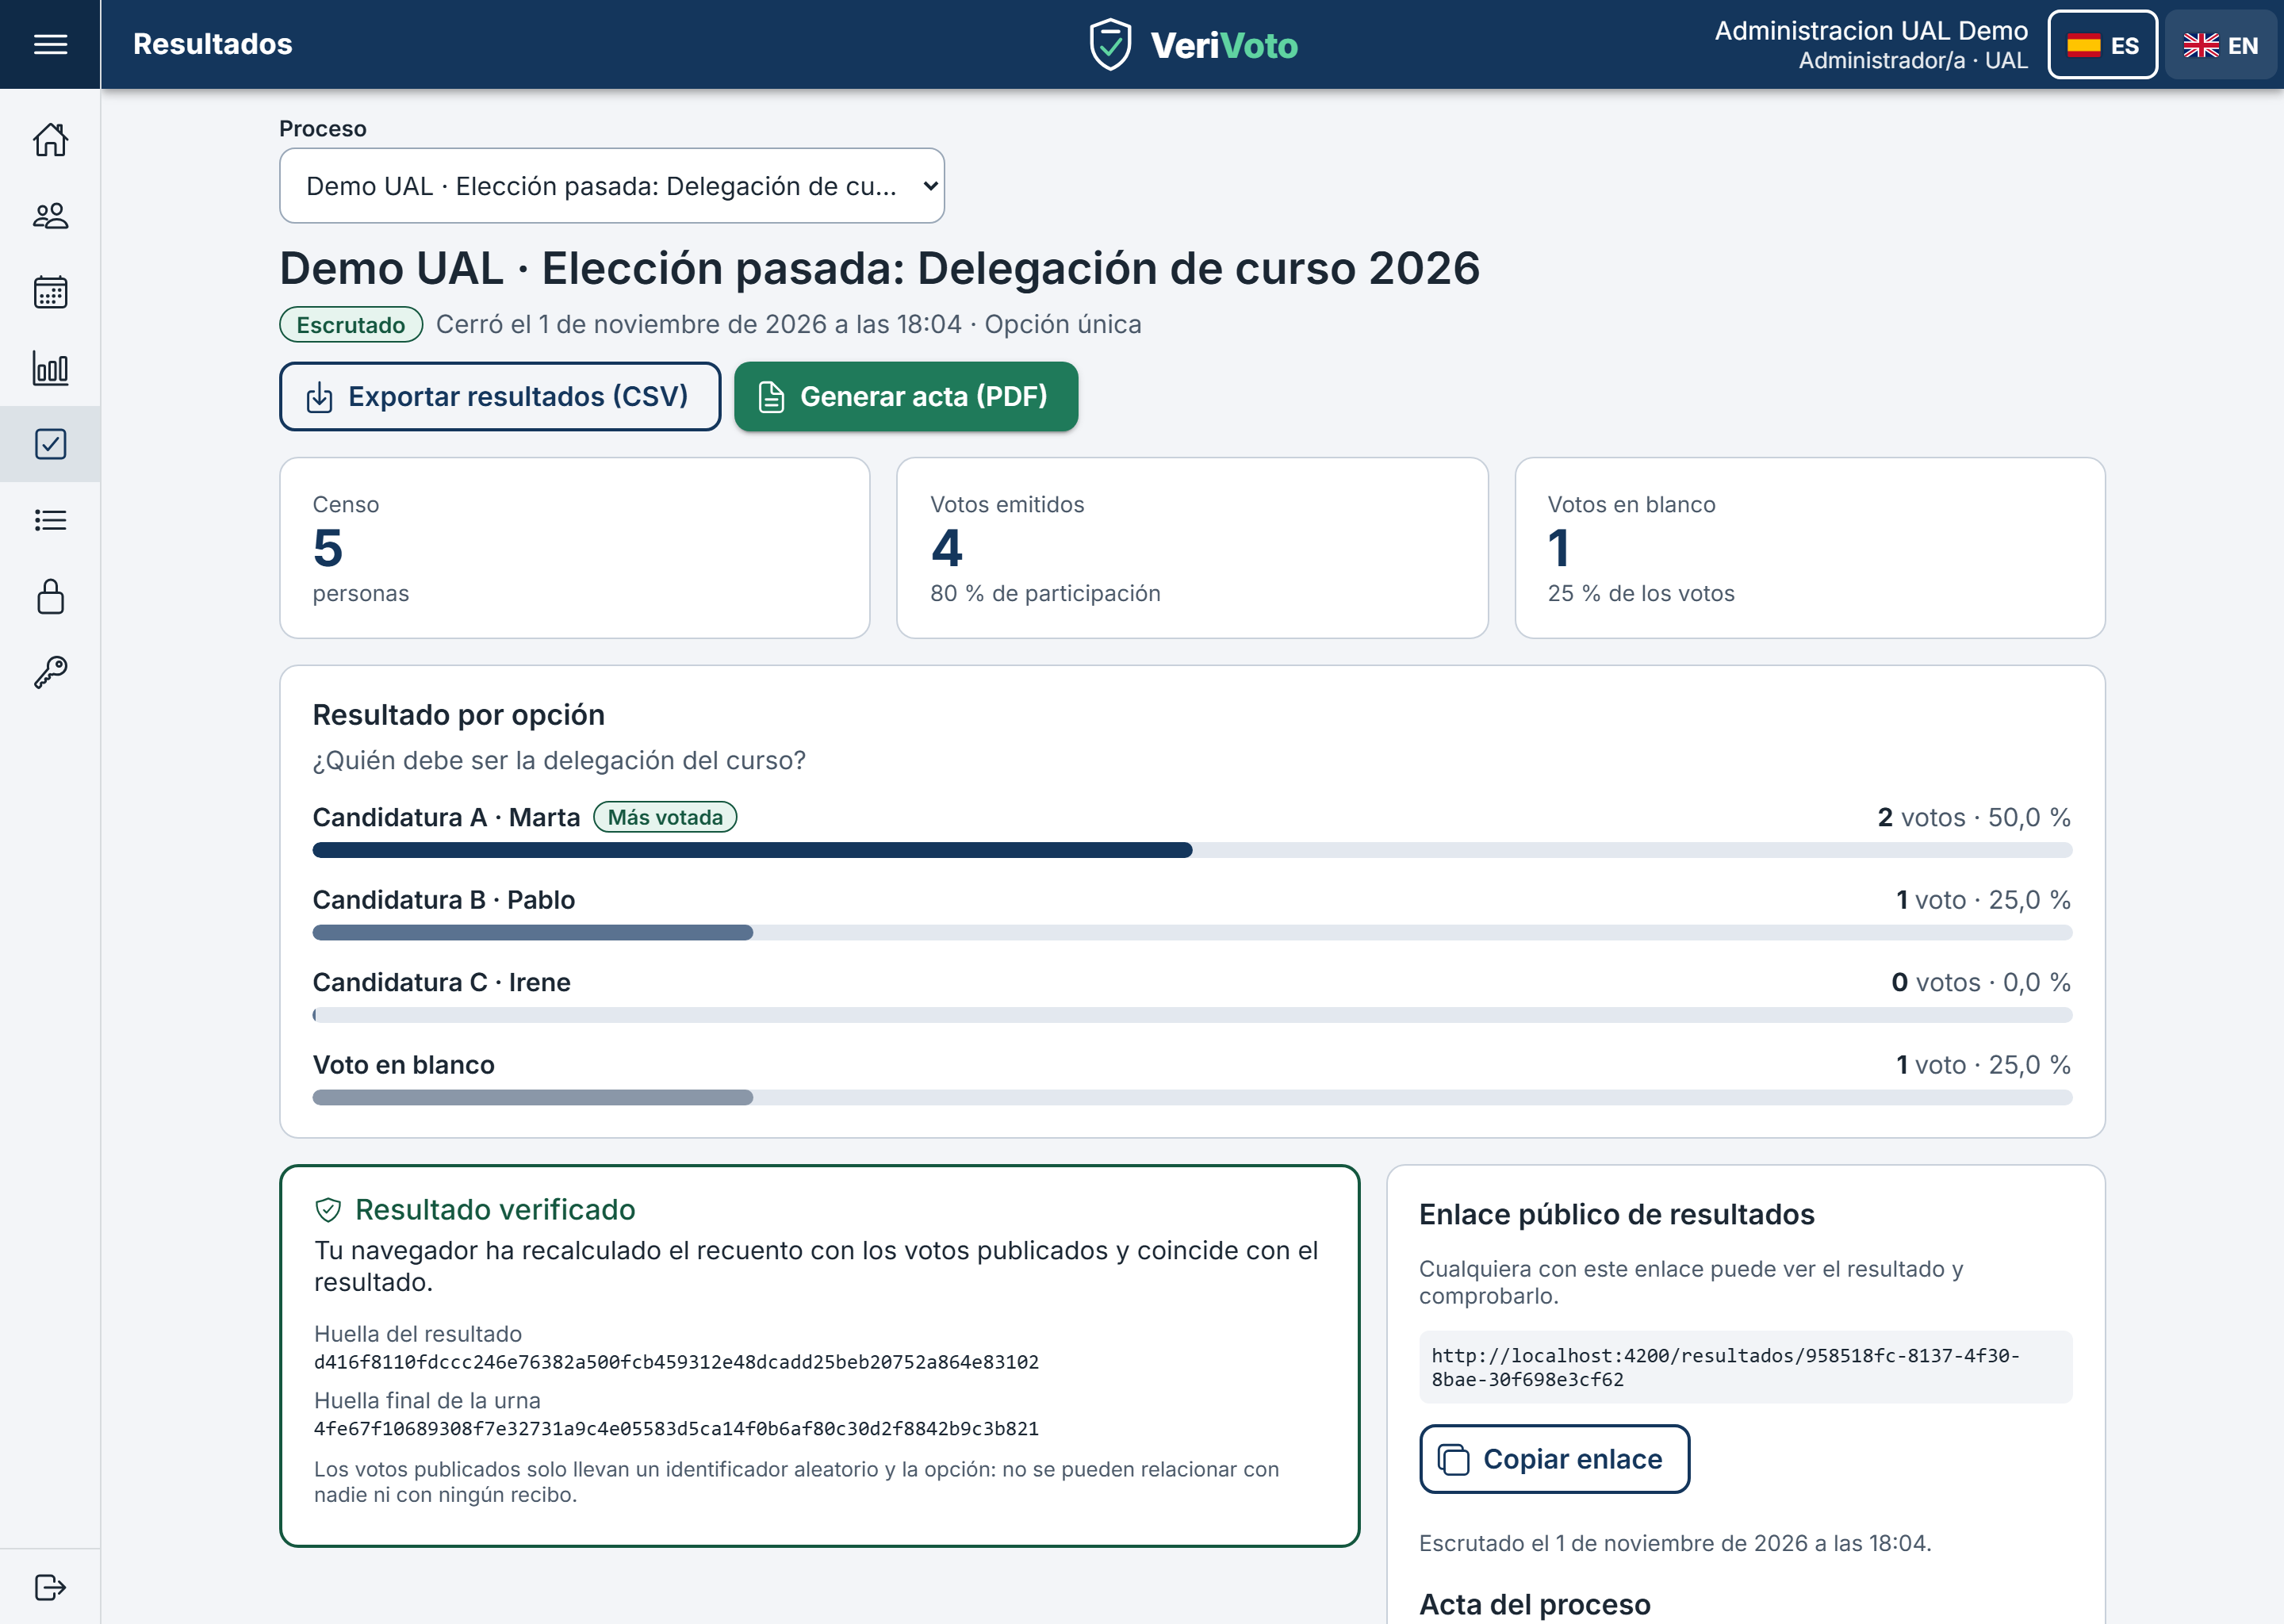
\includegraphics[width=\linewidth]{capturas/consola-resultados-es}\\
    \footnotesize Resultado, acta y huellas (RF-15, RF-16)
  \end{columns}
\end{frame}

% ---------------------------------------------------------------- 10
\section{Evaluación}
\begin{frame}{Calidad del código y seguridad}
  \begin{columns}[T]
    \column{0.24\textwidth}\cifra{312}{pruebas automáticas, 0 fallos\\(168 backend, 144 frontend)}
    \column{0.24\textwidth}\cifra{23}{de integración sobre PostgreSQL real}
    \column{0.24\textwidth}\cifra{212}{comprobaciones axe sin incumplimientos críticos ni serios}
    \column{0.24\textwidth}\cifra{>85\,\%}{cobertura del código nuevo (SonarQube)}
  \end{columns}
  \vspace{10pt}
  \begin{itemize}\small
    \item CI en GitHub Actions: pruebas, accesibilidad, Semgrep, Trivy, gitleaks, \texttt{npm audit}
    \item Modelo de amenazas STRIDE; límite de peticiones por IP y audiencia JWT exigida
    \item Cobertura global de líneas: 59,1\,\% backend y 42,0\,\% frontend (limitación declarada)
  \end{itemize}
\end{frame}

% ---------------------------------------------------------------- 11
\begin{frame}{Hipótesis: resultados}
  \footnotesize
  \begin{tabular}{@{}>{\raggedright\arraybackslash}p{0.21\textwidth}>{\raggedright\arraybackslash}p{0.36\textwidth}>{\raggedright\arraybackslash}p{0.36\textwidth}@{}}
    \toprule
    \textbf{Hipótesis} & \textbf{Criterio} & \textbf{Resultado}\\
    \midrule
    H1b · usabilidad del votante & 5 de 5 votan con recibo en \(\le\) 3 min; \(\ge\) 4 de 5 lo entienden & \textcolor{acierto}{\textbf{ACEPTADA}}: 5 de 5 (mediana 51 s); 5 de 5 entienden el recibo\\\addlinespace
    RNF-4 · administración & \(\ge\) 4 de 5 crean y programan un proceso en \(\le\) 10 min sin ayuda & \textcolor{acierto}{\textbf{ACEPTADO}}: 5 de 5, máximo 4 min\\\addlinespace
    H1a · accesibilidad & 0 críticos ni serios + revisión manual & \textcolor{pendiente}{\textbf{SIN DECISIÓN}}: parte automática favorable; manual no realizada\\\addlinespace
    H1c · rendimiento & 500 simultáneos, p95 \(<\) 2 s en 3 ejecuciones & \textcolor{fallo}{\textbf{RECHAZADA}}: p95 2,4--4,9 s; cadena íntegra\\
    \bottomrule
  \end{tabular}
  \vspace{6pt}
  \ualbloque{\footnotesize Con \(n = 5\) la evidencia es descriptiva, sin inferencia estadística. Los criterios no se cambiaron al ver los resultados.}
\end{frame}

% ---------------------------------------------------------------- 12
\section{Conclusiones}
\begin{frame}{Conclusiones}
  \begin{description}\small
    \item[RQ1] Un recibo de presencia y una página pública permiten explicar la verificación sin revelar el voto: 5 de 5 participantes la interpretaron bien.
    \item[RQ2] Separar participación y urna, sin identificadores ni horas por voto, con un token de un solo uso, controla la unicidad y reduce la vinculación.
    \item[RQ3] ISO/IEC 25010:2023 organiza los RNF y la evaluación; la evidencia cubre usabilidad e integridad, y queda incompleta en rendimiento y accesibilidad manual.
  \end{description}
  \vspace{4pt}
  \ualbloque{\small Los cuatro objetivos están implementados; la aceptación experimental es parcial y se declara como tal.}
\end{frame}

% ---------------------------------------------------------------- 13
\begin{frame}{Limitaciones y trabajo futuro}
  \begin{columns}[T]
    \column{0.48\textwidth}
    \textbf{Limitaciones}
    \begin{itemize}\small
      \item Solo en local, con datos sintéticos
      \item Rendimiento por debajo del objetivo
      \item Accesibilidad manual sin realizar
      \item SSO de gestión sin un proveedor externo real
      \item Muestras de cinco personas
    \end{itemize}
    \column{0.48\textwidth}
    \textbf{Trabajo futuro}
    \begin{itemize}\small
      \item Optimizar y repetir H1c
      \item Revisión con lector de pantalla
      \item Sustitución del voto (RF-11)
      \item Verificabilidad extremo a extremo y cifrado en cliente
      \item Despliegue con CSP, HSTS y secretos gestionados
    \end{itemize}
  \end{columns}
\end{frame}

% ---------------------------------------------------------------- 14
{
\setbeamertemplate{footline}{}
\begin{frame}[plain]
  \centering
  \vspace{1.2cm}
  {\color{ualoscuro}\Large\bfseries Gracias\par}
  \vspace{8pt}
  {\large Turno de preguntas\par}
  \vspace{18pt}
  {\small Saul David Ramos Pacheco · Máster Universitario en Ingeniería Informática · UAL\par}
  \vspace{12pt}
  
\includegraphics[height=1.4cm]{logos/escudocolor.png}
\end{frame}
}

% ================================================================ Reserva
\appendix
\section{Diapositivas de reserva}

\begin{frame}{Reserva: H1c, por qué no se alcanzó el rendimiento}
  \begin{columns}[T]
    \column{0.48\textwidth}
    \textbf{Lo medido} (11/11/2026, un equipo Windows)
    \begin{itemize}\small
      \item p95 de la emisión: 4852, 2402 y 4849 ms
      \item Votos aceptados: 222, 240 y 281 de 500
      \item Resto: conexiones rechazadas por el \emph{gateway}
      \item En las tres: cadena íntegra y recuento coherente
    \end{itemize}
    \column{0.48\textwidth}
    \textbf{Causas probables y siguiente paso}
    \begin{itemize}\small
      \item 500 conexiones a la vez, sin rampa
      \item Bloqueo del proceso para encadenar cada voto: se guardan de uno en uno
      \item Perfilar, ajustar colas y repetir en un entorno dimensionado, \textbf{sin cambiar el criterio}
    \end{itemize}
  \end{columns}
\end{frame}

\begin{frame}{Reserva: participación y trazabilidad}
  \begin{columns}[T]
    \column{0.5\textwidth}\centering
    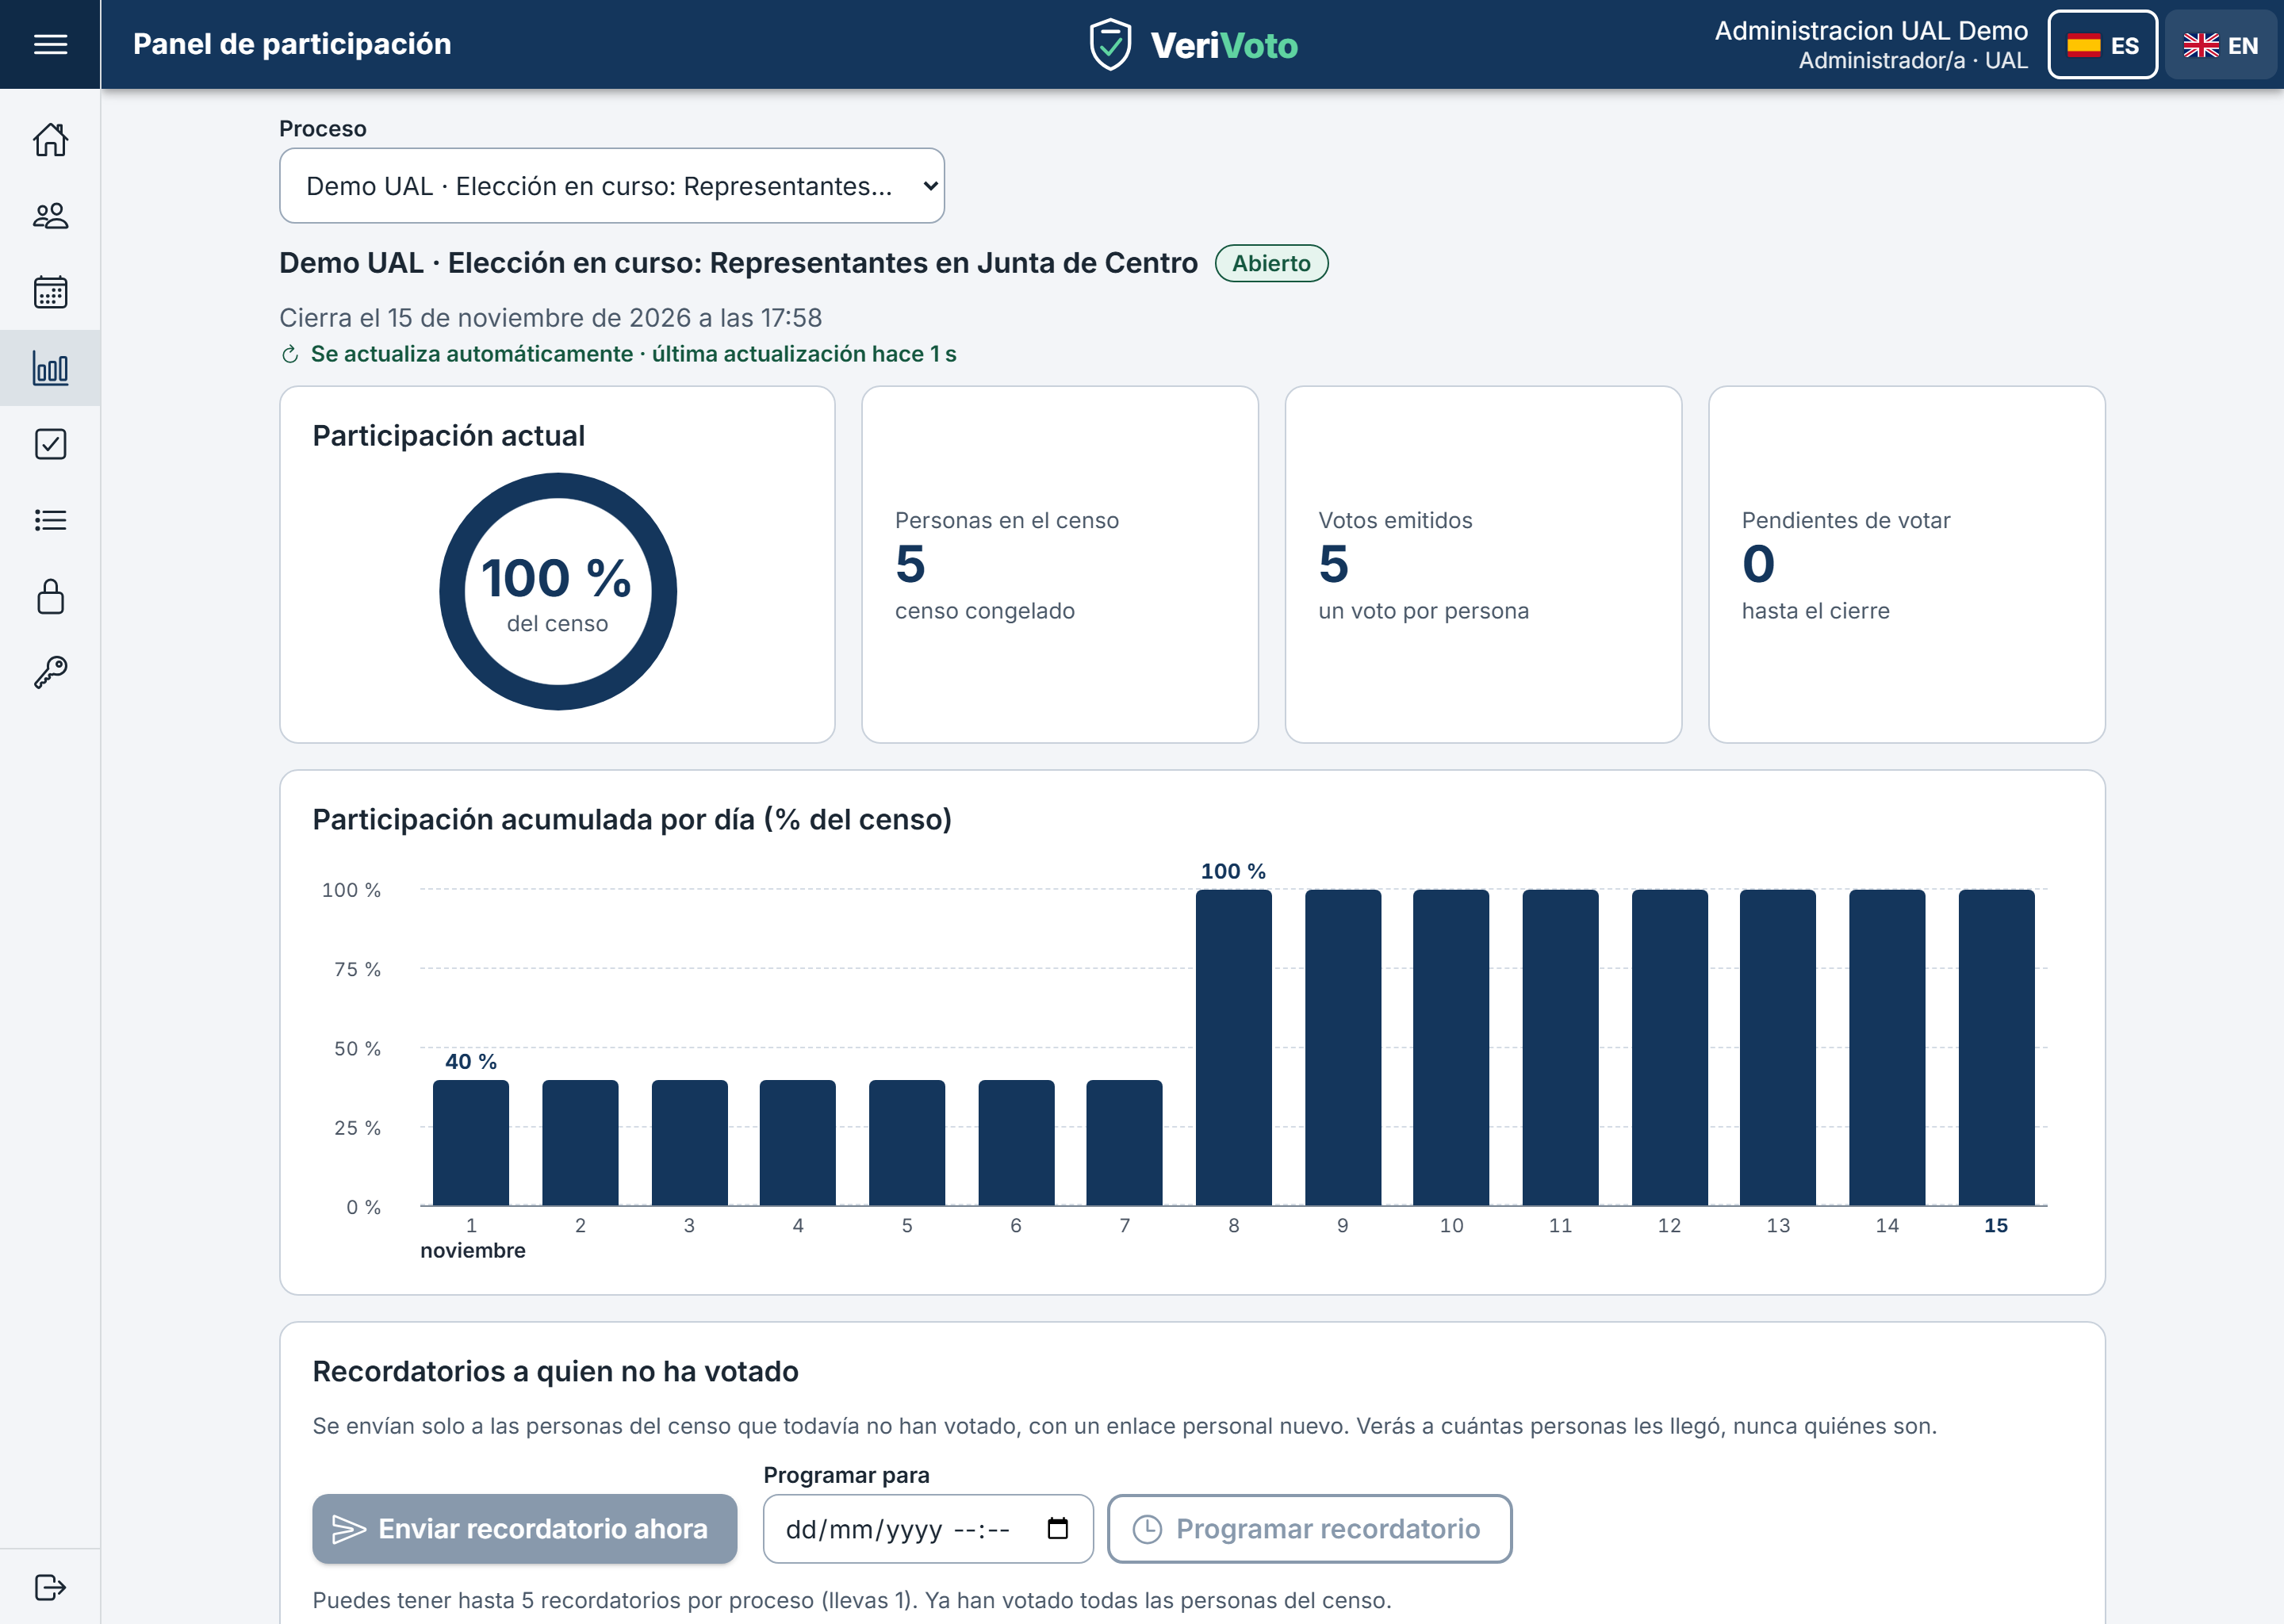
\includegraphics[width=\linewidth]{capturas/consola-participacion-es}\\
    \footnotesize Participación agregada, nunca quién votó (RF-14)
    \column{0.5\textwidth}\centering
    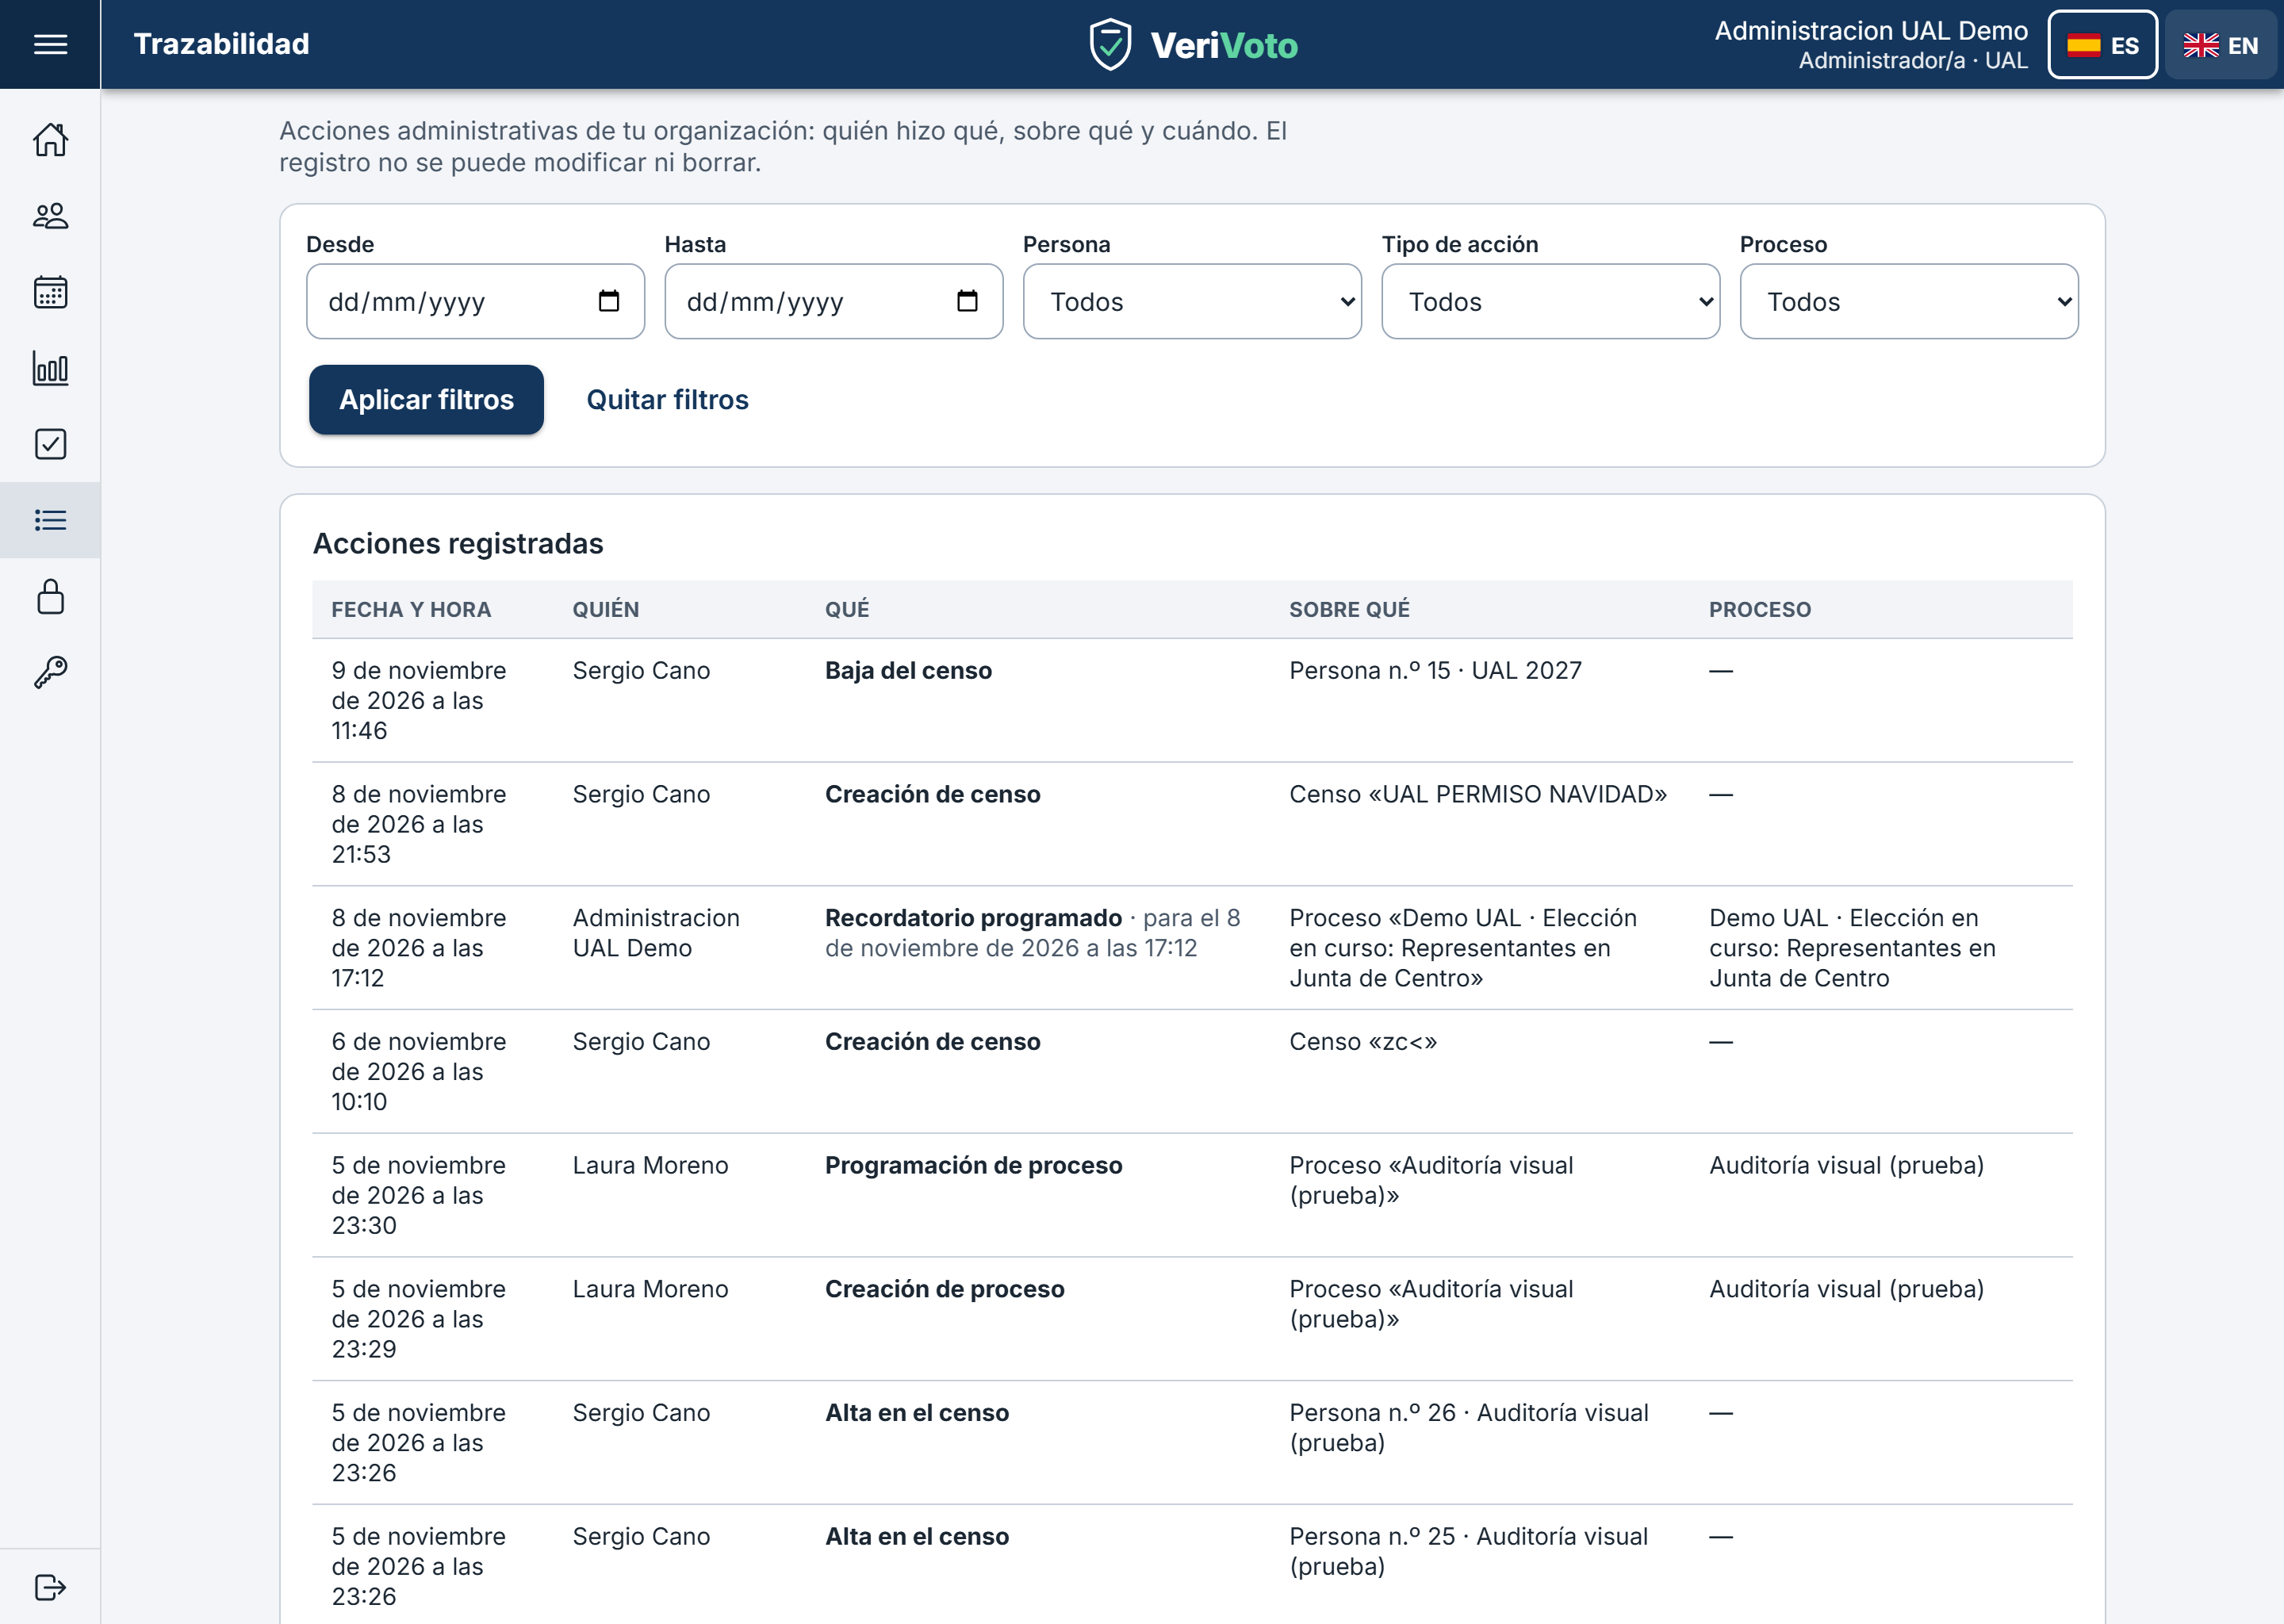
\includegraphics[width=\linewidth]{capturas/consola-trazabilidad-es}\\
    \footnotesize Acciones administrativas, solo añadir (RF-19)
  \end{columns}
\end{frame}

\begin{frame}{Reserva: decisiones de arquitectura}
  \small
  \begin{itemize}
    \item \textbf{Cinco servicios} (D-05): separación mínima que protege el secreto (identidad y urna aparte) sin multiplicar el despliegue.
    \item \textbf{REST síncrono + \emph{outbox}} en lugar de Kafka: menos piezas para un MVP local; entrega al menos una vez con reintentos.
    \item \textbf{Keycloak} para la gestión (contraseña + código por correo, SSO por organización); el votante entra con enlace y código propios.
    \item \textbf{Hexagonal}: el dominio no depende de Spring; reglas comprobadas con ArchUnit.
    \item \textbf{Multi-tenant} por columna \texttt{organization\_id} y filtro en cada consulta; probado con dos organizaciones por HTTP.
  \end{itemize}
\end{frame}

\begin{frame}{Reserva: arquitectura objetivo frente a implementada}
  \centering
  \resizebox{!}{0.8\textheight}{\diagrama{arquitectura_componentes_saas_votacion}}
\end{frame}

\begin{frame}{Reserva: amenazas principales (STRIDE)}
  \footnotesize
  \begin{tabular}{@{}>{\raggedright\arraybackslash}p{0.22\textwidth}>{\raggedright\arraybackslash}p{0.36\textwidth}>{\raggedright\arraybackslash}p{0.34\textwidth}@{}}
    \toprule
    \textbf{Amenaza} & \textbf{Control} & \textbf{Estado}\\
    \midrule
    Votar dos veces & Token de un solo uso, restricción única en la urna & Probado con 20 envíos simultáneos\\
    Vincular votante y voto & Bases separadas, sin hora ni identidad por voto & Revisado (esquema y registros)\\
    Alterar la urna & Cadena de huellas, tabla solo añadir & Escrutinio bloqueado si se rompe\\
    Token de otro cliente & Audiencia \texttt{verivoto-api} exigida & Implementado\\
    Inundar códigos o votos & Límite por enlace y por IP en el \emph{gateway} & Implementado\\
    \bottomrule
  \end{tabular}
\end{frame}

\begin{frame}{Reserva: plan previsto y ejecución}
  \small
  \begin{itemize}
    \item Desarrollo P0--P6 terminado antes de su ventana prevista.
    \item P7 (pruebas y medición) cerrado el 15/11/2026: H1b el 09/11, H1c el 11/11, RNF-4 el 13/11.
    \item P8 (memoria) en revisión final; entrega el 27/01/2027.
    \item Experiencia previa aplicada: tres años de microservicios Java en banca y las Prácticas Externas.
  \end{itemize}
\end{frame}

\end{document}
